\documentclass[11pt]{article}

\usepackage[final]{acl}

% Standard package includes
\usepackage{times}
\usepackage{latexsym}
\usepackage[T1]{fontenc}
\usepackage[utf8]{inputenc}
\usepackage{microtype}
% \usepackage{inconsolata} % removed: font not available
\usepackage{graphicx}
\usepackage{booktabs}
\usepackage{array}
\usepackage{url}
\hyphenpenalty=10000
\title{Counterfactual Visual Analytics for Targeted Student Interventions}

\author{Yiming Xiao \\
  Texas A\&M University \\
  UIN: 835009298\\
  \texttt{yxiao@tamu.edu} \\\And
  Yi-Hsin Chiang \\
  Texas A\&M University \\
  UIN:137001082 \\
  \texttt{yihsin.chiang@tamu.edu} \\}

\begin{document}
{\makeatletter\acl@finalcopytrue
  \maketitle
}

\begin{abstract}
Academic dashboards used in higher education today are largely descriptive tools: they report what has already happened but offer little guidance on what instructors or advisors should do next. This paper proposes \textit{Counterfactual Visual Analytics for Targeted Student Interventions}, an interactive visualization system that combines multiple linear regression with bootstrapped confidence intervals and real-time counterfactual ``what-if'' exploration. By letting instructors manipulate actionable variables such as tutoring sessions and attendance via interactive sliders, the system instantly updates a predicted exam-score distribution, visually comparing a student's current trajectory against an intervened scenario. We anticipate that the tool will help academic advisors formulate intervention plans faster and with greater confidence than existing spreadsheet-based workflows.
\end{abstract}

% -----------------------------------------------------------------------
\section{Introduction}
% -----------------------------------------------------------------------

Early identification of at-risk students and timely intervention are two of the most effective levers available to higher-education institutions for improving retention and academic outcomes. Yet the dashboards most commonly used by instructors today are fundamentally backward-looking. They surface grades, attendance records, and class averages after the fact, giving educators a clear picture of \textit{what happened} but no systematic way to reason about \textit{what to do next}. A professor who notices a student trending toward failure is left to rely on intuition or informal heuristics when deciding whether to recommend additional tutoring, encourage better attendance, or suggest improved sleep habits.

This gap between descriptive reporting and actionable guidance is the core problem we address. We propose a causal-predictive visual analytics system that moves beyond historical summaries to support forward-looking, evidence-based decision making. The key idea is counterfactual reasoning: given a student's current profile, the system asks ``What would the predicted outcome be \textit{if} we changed variable $X$ by a certain amount?'' and renders the answer as an immediately interpretable visual comparison.

Concretely, we fit a multiple linear regression model on a student performance dataset containing 20 features per student. The predictions are accompanied by confidence intervals so that advisors can see not just a point estimate but the uncertainty around it. An interactive intervention panel exposes sliders for actionable variables. Moving a slider instantly redraws a predicted score distribution on top of the student's baseline, making the expected benefit of each intervention immediately visible.

% -----------------------------------------------------------------------
\section{Related Work}
\label{sec:related}
% -----------------------------------------------------------------------

\paragraph{Learning analytics and dashboards.}
The field of learning analytics has produced a wide range of tools aimed at monitoring and improving student outcomes \cite{siemens2013learning}. Most deployed dashboards, however, remain in the descriptive analytics tier: they aggregate log data, attendance, and grade records into visualizations that help instructors see where students stand, but they do not prescribe interventions \cite{papamitsiou2014learning}. Our work is motivated by the observation that bridging descriptive and prescriptive analytics requires an explicit model of how changing behavior leads to changed outcomes.

\paragraph{Prediction models for student performance.}
Machine learning models for predicting student success have been extensively studied \cite{romero2020educational}. \citet{asselman2023} demonstrate that gradient-boosted models such as XGBoost achieve strong predictive accuracy, and \citet{khalaf2025} show that ensemble regressors further improve performance. A recurring theme in this literature is that accuracy alone is insufficient: without interpretability, educators cannot act on model outputs. This motivates our choice of multiple linear regression, whose coefficients are directly interpretable as marginal effects of each feature on the predicted exam score.

% \paragraph{Explainable AI in education.}
% The need for interpretable models in educational contexts has driven adoption of explainability techniques such as SHAP and LIME \cite{shapley2022,choi2025}. \citet{ben2022} show that SHAP values provide a detailed view of each variable's influence on academic performance and can be integrated into interactive visualization systems for scenario exploration. While these methods are post-hoc and model-agnostic, they typically explain a single prediction rather than enabling interactive simulation. Our system takes a different approach: by using a transparent linear model from the outset, coefficients are directly readable and counterfactual changes can be computed in closed form, enabling real-time interaction.

\paragraph{Counterfactual explanations in education.}
Counterfactual explanations have attracted growing interest in educational data mining \cite{bunay2026}. \citet{tsiakmaki2021} present a case study showing that interpretable counterfactual explanations can identify critical factors for student success and enable personalized educational strategies. \citet{afrin2023} use Diverse Counterfactual Explanations (DiCE) to show that changes in study behavior could shift students from failing to passing, validated through a user study with educators. \citet{susnjak2022} demonstrate the use of predictive and counterfactual learning analytics panels to estimate academic success. A systematic review by \citet{bunay2026} finds that counterfactual methods are increasingly applied to student dropout and retention, but notes that no consensus exists on which generation method is most suitable. Our proposal extends this line of work by embedding counterfactual generation inside an interactive visual analytics interface with uncertainty visualization.

\paragraph{Visual analytics for dropout and at-risk students.}
Several systems have explicitly targeted at-risk student identification through visualization. \citet{sdavis2022} introduce SDA-Vis, a system that supports counterfactual exploration of student dropout dynamics across academic, social, and economic variables. \citet{zhang2023} combine a CNN-LSTM model with counterfactual explanations to visually analyze dropout behavior patterns in online learning environments, quantifying the impact of behavioral changes on dropout probability. Both systems demonstrate the value of embedding counterfactual reasoning inside a visual interface, which is the approach we pursue for the general exam-score prediction setting.

% -----------------------------------------------------------------------
\section{Dataset}
\label{sec:dataset}
% -----------------------------------------------------------------------

We use the \textit{Student Academic Performance Dataset} by Ayesha Siddiqa, publicly available on Kaggle. The dataset records 20 features per student and includes the final exam score as the target variable. Table~\ref{tab:features} summarizes the features by category, illustrating their data types and counterfactual actionability.


\begingroup
\renewcommand{\arraystretch}{1.5}
\begin{table*}[h]
\centering
\small
\begin{tabular}{p{3.0cm} p{6cm} p{1.5cm} p{3.5cm}}
\toprule
\textbf{Category} & \textbf{Example Variables} & \textbf{Type} & \textbf{Actionability} \\
\midrule
Academic History & Previous\_Scores, Exam\_Score & Numeric & Immutable (baseline) \\
Student Behavior & Hours\_Studied, Attendance & Numeric & High (direct) \\
Lifestyle \& Habits & Sleep\_Hours, Extracurricular & Num./Cat. & Moderate (counseling) \\
Environment \& Support & Tutoring\_Sessions, Parental\_Involvement & Cat. & Partial (resources) \\
\bottomrule
\end{tabular}
\caption{Feature categories, example variables, data types, and counterfactual actionability.}
\label{tab:features}
\end{table*}
\endgroup


Figure~\ref{fig:corr} shows the Pearson correlation matrix for the main numeric features. The strongest correlates of Exam\_Score are Attendance ($r = 0.58$) and Hours\_Studied ($r = 0.45$), followed by Previous\_Scores, Access\_to\_Resources, and Tutoring\_Sessions. The low inter-feature correlations indicate that multicollinearity is not a serious concern for the regression model. Importantly, no single factor comes close to explaining the full variance in exam scores, motivating a multivariate model that weighs all 20 factors together.

\begin{figure}[h]
  \centering
  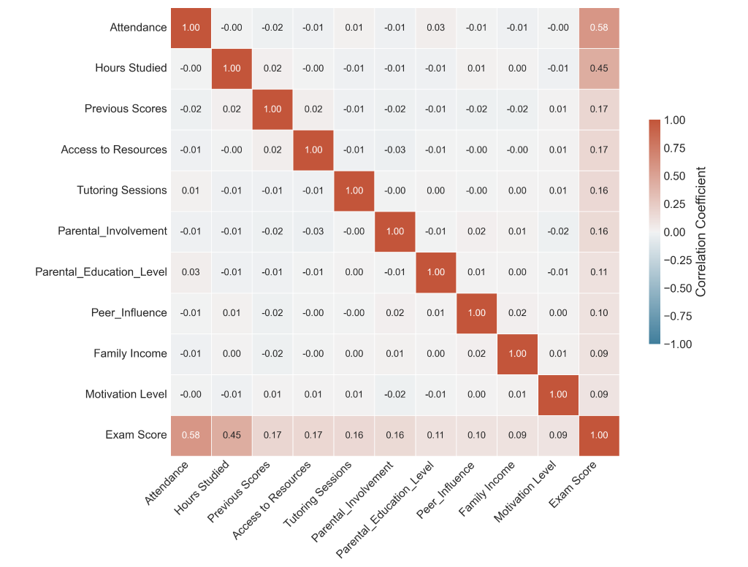
\includegraphics[width=\columnwidth]{corr.png}
  \caption{Pearson correlation matrix for numeric student features.}
  \label{fig:corr}
\end{figure}

A key observation is that current descriptive dashboards, such as the attendance-vs.-exam-score scatter plot shown in Figure~\ref{fig:scatter}, reveal correlational patterns but provide no guidance on which intervention will actually help a specific struggling student.

\begin{figure}[h]
  \centering
  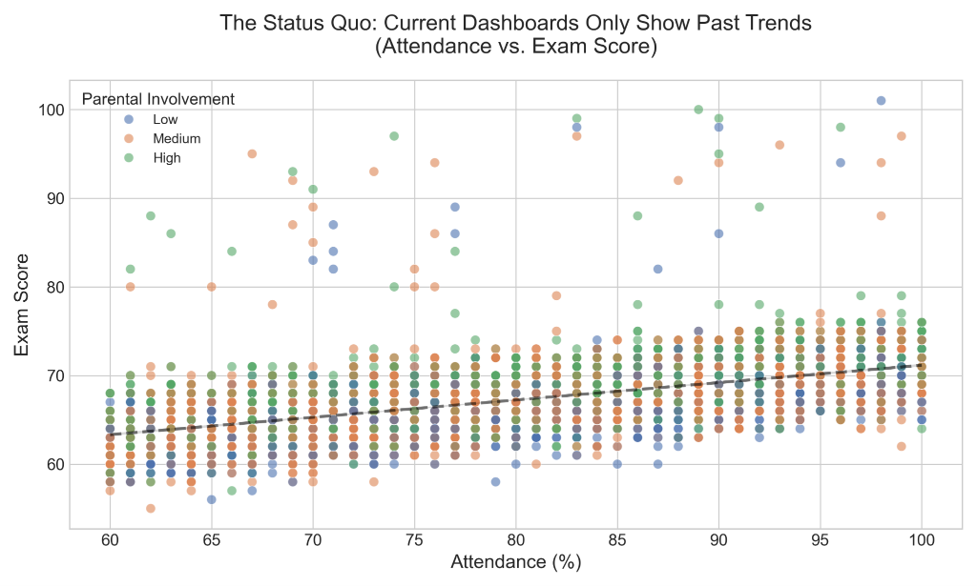
\includegraphics[width=\columnwidth]{scatter.png}
  \caption{Attendance vs.\ Exam Score scatter plot colored by Parental Involvement level. Representative of the backward-looking descriptive dashboards that currently dominate educational reporting.}
  \label{fig:scatter}
\end{figure}

% -----------------------------------------------------------------------
\section{System Design}
\label{sec:system}
% -----------------------------------------------------------------------

\subsection{Statistical Model}

We fit a multiple linear regression model of the form
\[
  \hat{y} = \beta_0 + \sum_{j=1}^{p} \beta_j x_j,
\]
where $\hat{y}$ is the predicted exam score and $x_1, \ldots, x_p$ are the 20 student features (with categorical variables one-hot encoded). The model is trained using ordinary least squares. We apply the bootstrap ($B = 1000$ resamples) to obtain confidence intervals around each coefficient and each individual prediction, yielding a predicted score \textit{distribution} rather than a point estimate.

A key design choice is to favor a transparent model over a more complex black-box predictor. Each coefficient $\beta_j$ is directly interpretable as ``an additional tutoring session per week is associated with $+\beta_j$ exam-score points.'' This transparency is essential for user trust and allows advisors to reason about the practical meaning of each slider adjustment.

\subsection{Visualization Interface}

The proposed interface, Figure~\ref{fig:ui}, centers on a \textit{counterfactual ``what-if'' plot} with two overlapping density curves for a selected student:

\begin{itemize}
  \item \textbf{Baseline (red):} the predicted distribution given the student's current feature values. The expected score and probability of falling below the failing threshold (score $< 60$) are shown explicitly.
  \item \textbf{Simulation (green):} the predicted distribution under the user's proposed intervention. The shift in expected score and the reduction in failure probability are immediately visible as the green curve moves right.
\end{itemize}

An \textit{Intervention Simulator} panel below the plot exposes interactive sliders for actionable variables and dropdowns for categorical variables. Moving a slider in real time redraws the green distribution without requiring a button press.

\begin{figure}[h]
  \centering
  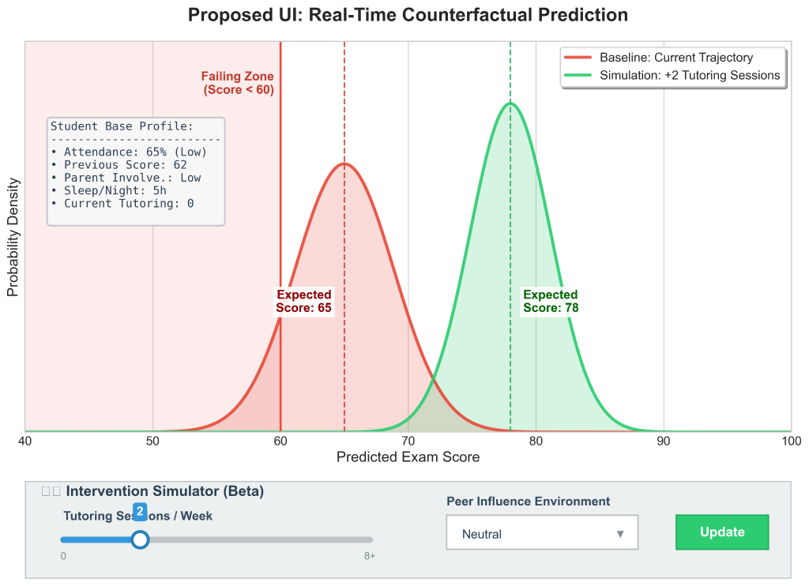
\includegraphics[width=\columnwidth]{ui.png}
  \caption{Proposed visualization interface. The red curve shows the baseline predicted score distribution; the green curve shows the distribution after simulating an intervention (e.g., $+2$ tutoring sessions/week). The failing zone (score $<60$) is shaded in red.}
  \label{fig:ui}
\end{figure}

The frontend will be implemented in D3.js, which provides the flexibility needed for custom density curves, dynamic axis updates, and linked slider interactions. Statistical computations (regression fitting, bootstrapping, prediction) will be performed in Python.

\begin{table*}[h]
\centering
\small
\begin{tabular}{cl}
\toprule
\textbf{Weeks} & \textbf{Milestone} \\
\midrule
1--2 & User interviews; data preprocessing; regression model fitting and bootstrap validation \\
3--4 & Frontend dashboard implementation in D3.js (static prototype) \\
5--6 & Backend integration; bootstrapped CI; slider interactions \\
7--8 & User evaluation study; results analysis; final report \\
\bottomrule
\end{tabular}
\caption{8-week development and evaluation timeline.}
\label{tab:timeline}
\end{table*}

% -----------------------------------------------------------------------
\section{Target Users and Requirements}
\label{sec:users}
% -----------------------------------------------------------------------

The primary target users are \textbf{university instructors, professors, and academic advisors} responsible for monitoring student progress and deciding when and how to intervene. These users typically have limited time per student and need to prioritize their attention efficiently.

To gather concrete design requirements, we plan to conduct \textbf{semi-structured interviews} with 2--3 instructors or academic advisors following a protocol that includes: (1)~\textit{context setting}: ``Walk me through how you currently identify and advise a struggling student''; (2)~\textit{pain point elicitation}: ``What information do you wish you had but currently lack?''; (3)~\textit{wireframe walkthrough}: showing low-fidelity mockups of the proposed interface; and (4)~\textit{variable mapping}: ``Which of these 20 factors do you think you can realistically change, and which are outside your control?''

The interviews serve two purposes. First, they validate the actionability taxonomy in Table~\ref{tab:features}, ensuring that the sliders correspond to variables that advisors actually believe they can influence. Second, they surface additional requirements, such as whether advisors need to compare multiple students simultaneously or export intervention plans as reports.

% -----------------------------------------------------------------------
\section{Evaluation Plan and Timeline}
\label{sec:evaluation}
% -----------------------------------------------------------------------

\subsection{Evaluation Design}

We will conduct a \textbf{controlled usability study} comparing two conditions: a \textbf{baseline} in which participants use a standard spreadsheet (Excel) containing the student dataset with no model outputs, and a \textbf{system} condition in which participants use the proposed interactive dashboard. We will measure two primary outcomes:

\begin{enumerate}
  \item \textbf{Time-to-Decision:} elapsed time from task start to committing to an intervention plan, measured via stopwatch.
  \item \textbf{Confidence Level:} self-reported 1--10 Likert scale asking ``How confident are you in your intervention plan?''.
\end{enumerate}

Secondary measures include the number and quality of distinct interventions proposed, and qualitative feedback from a brief post-task interview.

\subsection{Development Timeline}

Table~\ref{tab:timeline} presents the planned 8-week development schedule.



% -----------------------------------------------------------------------
\section{Expected Results}
\label{sec:results}
% -----------------------------------------------------------------------

We expect the system to produce three categories of measurable benefit.

\paragraph{Faster intervention planning.} By surfacing a model-backed prediction and enabling one-click what-if exploration, the system should substantially reduce the cognitive overhead of identifying the most impactful intervention for a given student, yielding a meaningful reduction in time-to-decision relative to the spreadsheet baseline.

\paragraph{Higher advisor confidence.} The transparent coefficient display (showing, for example, that attendance contributes 0.58 points per percentage point) gives advisors an evidence base for their recommendations. Combined with the visual uncertainty representation (the width of the predicted distribution), this is expected to increase self-reported confidence on the 1--10 scale.

\paragraph{Improved trust in institutional AI.} Prior work has found that counterfactual explanations increase user trust in model recommendations when the explanations are actionable and realistic \cite{afrin2023,tsiakmaki2021}. By restricting sliders to variables with high or moderate actionability, our system avoids recommending interventions advisors cannot implement (e.g., changing a student's family income), further grounding trust in practical reality. Over time, higher advisor confidence and more targeted interventions are expected to contribute positively to student retention rates.

% -----------------------------------------------------------------------
\bibliography{references}
\end{document}
